%!TeX root = ../paper-2024-cmpb-llm-chatbot-biomed.tex
\begin{figure}[!ht]
    \ContinuedFloat
    \centering
    \begin{subfigure}[b]{0.49\textwidth}
        \centering
        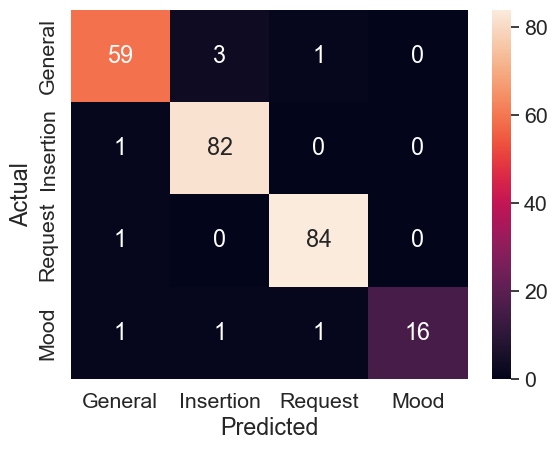
\includegraphics[width=\textwidth]{figures/confusion_matrices/nas_bert.png}
        \caption{ML.NET~2.0 framework}
        \label{fig:cm-nas-bert}
    \end{subfigure}
    \hfill
    \begin{subfigure}[b]{0.49\textwidth}  
        \centering 
        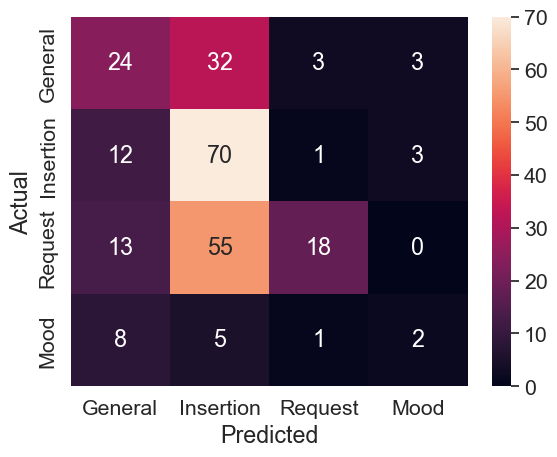
\includegraphics[width=\textwidth]{figures/confusion_matrices/alfred.png}
        \caption{Alfred}
        \label{fig:cm-alfred}
    \end{subfigure}
    \vskip\baselineskip
    \begin{subfigure}[b]{0.49\textwidth}  
        \centering 
        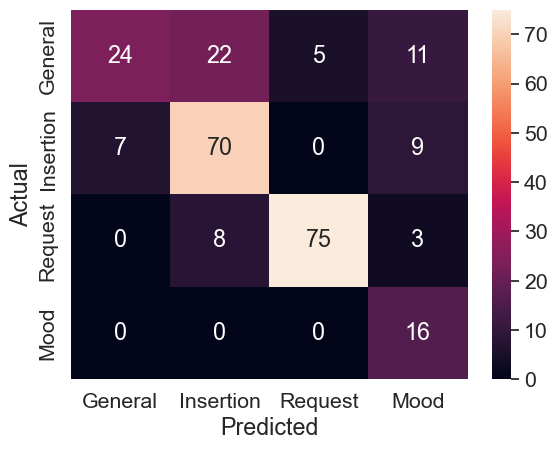
\includegraphics[width=\textwidth]{figures/confusion_matrices/llama2_70b.png}
        \caption{Llama2 70b}
        \label{fig:cm-llama70}
    \end{subfigure}
    \hfill
    \begin{subfigure}[b]{0.49\textwidth}   
        \centering 
        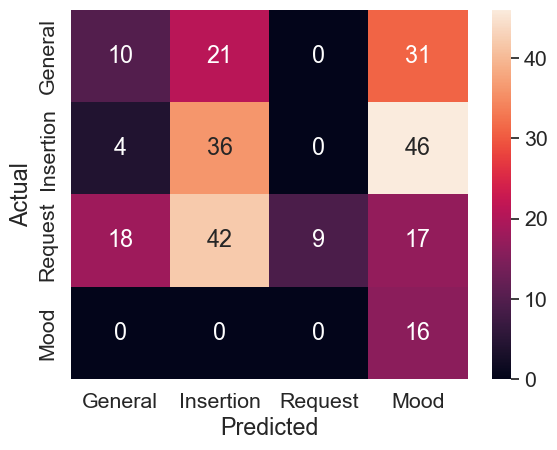
\includegraphics[width=\textwidth]{figures/confusion_matrices/llama2_13b.png}
        \caption{Llama2 13b}
        \label{fig:cm-llama13}
    \end{subfigure}
    \caption{Confusion matrices for the classification phase.}
    \label{fig:cm1}
\end{figure}
\begin{figure}[!ht]
    \ContinuedFloat
    \centering
    \begin{subfigure}[b]{0.49\textwidth}   
        \centering 
        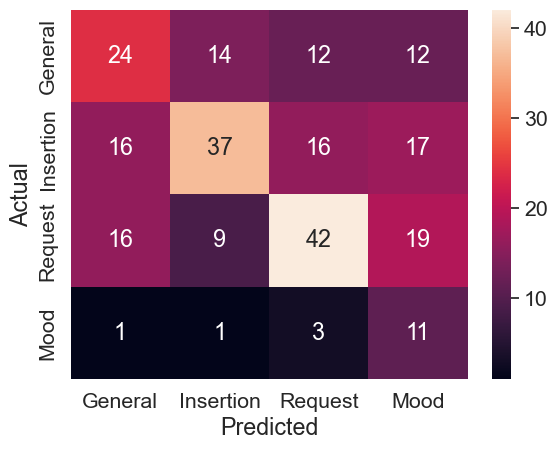
\includegraphics[width=\textwidth]{figures/confusion_matrices/llama2_7b.png}
        \caption{Llama2 7b}
        \label{fig:cm-llama7}
    \end{subfigure}
    \hfill
    \begin{subfigure}[b]{0.49\textwidth}   
        \centering 
        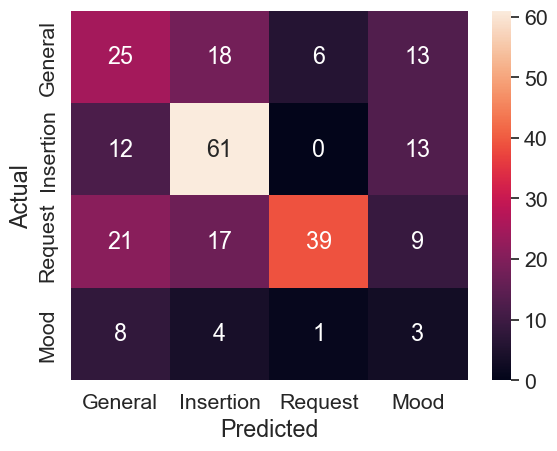
\includegraphics[width=\textwidth]{figures/confusion_matrices/mistral.png}
        \caption{Mistral}
        \label{fig:cm-mistral}
    \end{subfigure}
    \vskip\baselineskip
    \begin{subfigure}[b]{0.49\textwidth}   
        \centering 
        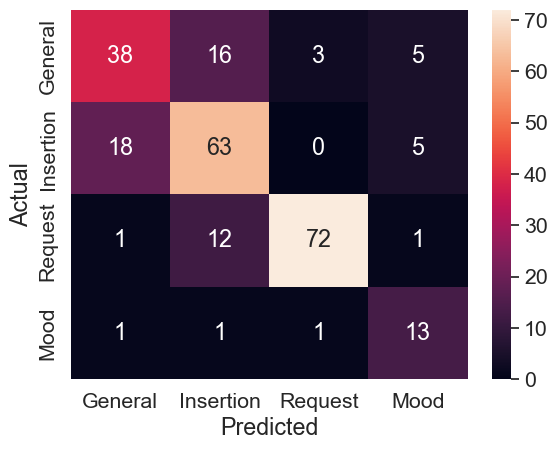
\includegraphics[width=\textwidth]{figures/confusion_matrices/mixtral.png}
        \caption{Mixtral}
        \label{fig:cm-mixtral}
    \end{subfigure}
    \caption{Confusion matrices for the classification phase.}
    \label{fig:cm2}
\end{figure}